\chapter{Design}
\label{c:design}

Hier beschreibst du High-Level deine Ideen und begründest die Auswahl der implementierten Vulnerabilities. Das kann zum Beispiel so aussehen:

% Struktur
\section{System Architecture}

\subsection{System Architecture Overview}

A modular, multi-app system architecture is used for the overarching structure of this Android project \todo{Maybe replace this "this Android project" wording with something better}. The implemented MASWE vulnerabilities are grouped by their respective MASVS category. This means that all implemented vulnerabilities of the category MASVS-STORAGE are part of the same module \texttt{maswe\_storage}, whereas the vulnerabilities from the MASVS-CRYPTO category make up their own \texttt{maswe\_crypto} module. 

Each module is its own Gradle Module, with its own AndroidManifest, activities, services, backup rules, and launcher activity. The advantage of this is a clean and structured separation of the different implementations by category. The categories can be tested and used independently from each other, and vulnerabilities that affect the AndroidManifest are contained to affect only other vulnerabilities of the same category, instead of all of them. Without this, a MASVS-PLATFORM vulnerability that sets the app to debuggable in the AndroidManifest would result in all vulnerabilities having to include this debuggable vulnerability.

To minimize the amount of redundancies we use a Shared-Library approach. This means that all independent MASVS app modules make use of the same \texttt{common} Android library module, which has a \texttt{res} folder containing the resource values shared by all apps. This includes values in regards to layout spacing, strings, string font sizes, and color values. The \texttt{common} library module also includes layouts shared by all apps and asbtract activity templates, as discussed in the next subsection. A high-level diagram of this architecture is shown in \ref{fig:highLevelViewSystemArchitecture}.

\begin{figure}[htbp]
  \centering
  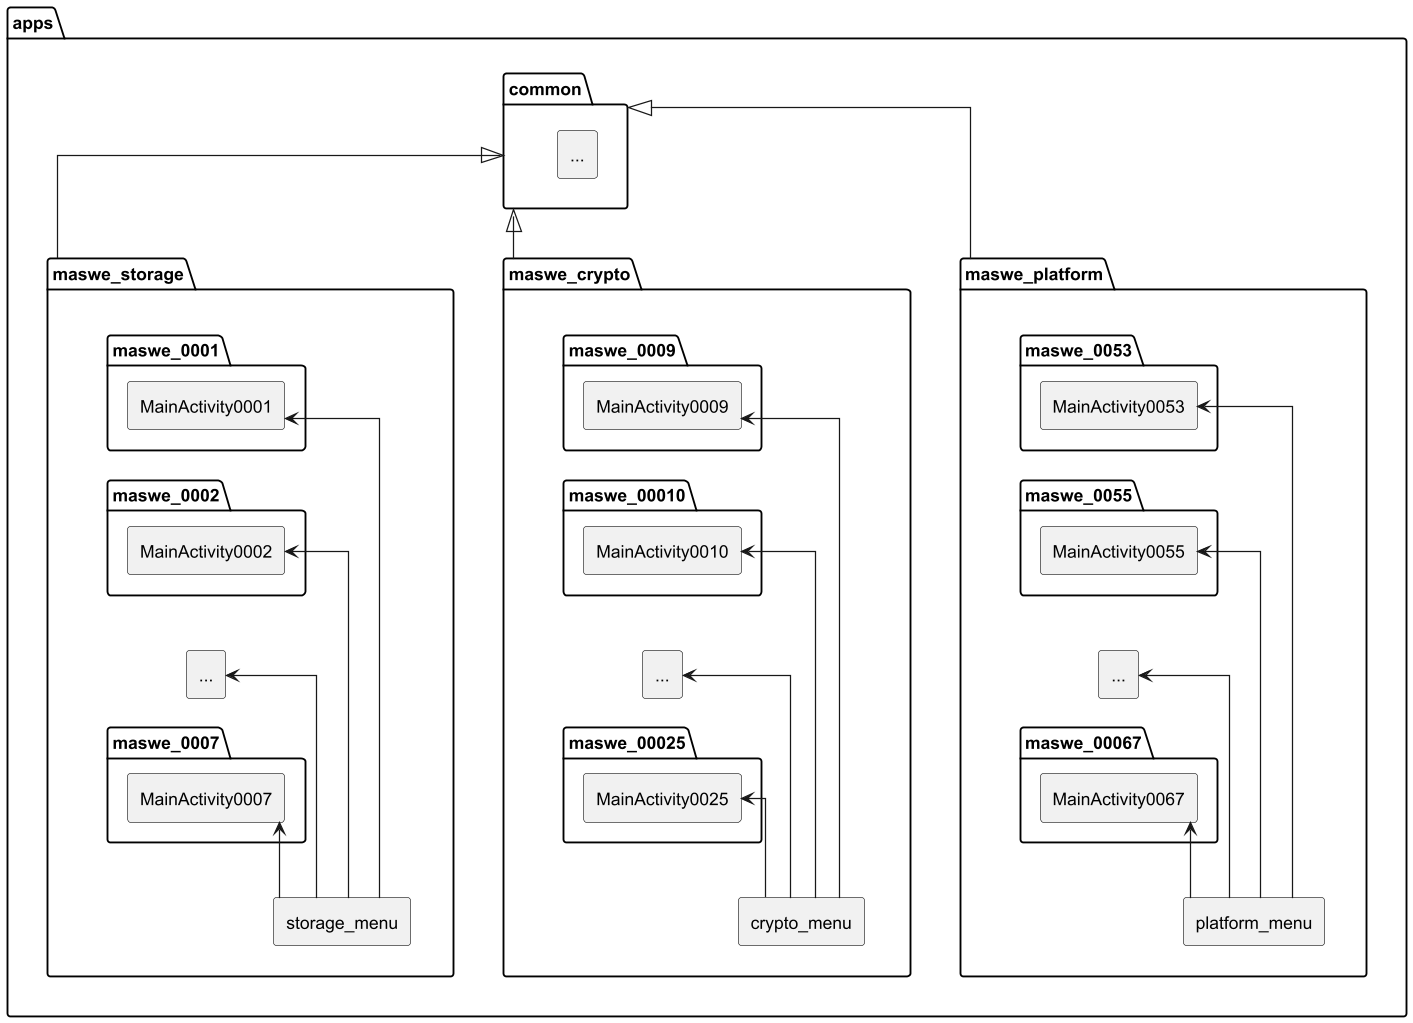
\includegraphics[width=1.0\textwidth]{dev_documents/BA_Thesis_Kronig/figures/diagrams/high_level_view_system_architecture.png}
  \caption{ \todo{Add image caption} }
  \label{fig:highLevelViewSystemArchitecture}
\end{figure}



\subsection{Feature-oriented Structure after OWASP MASVS}

Each app module is structured as follows. The launcher activity functions as the overview and hub from which all implemented vulnerabilities of the respective category can be chosen from. The vulnerabilities themselves are grouped into separate packages. These packages include all activities, services and other Java files that are part of the vulnerability's code. This includes for all vulnerabilties: a main activity serving as the vulnerability's starting point, as well as a \texttt{RegisterActivity.java}, \texttt{LoginActivity.java} and a \texttt{ProfileActivity.java}, that are used for user registration and login. This architecture is extended with other files depending on the vulnerability and its implementation, such as an \texttt{EncryptionHandler.java} which deals with cryptographic services.

This architecture further reinforces the clean separation and structure of the Android project. We package and isolate the code for each vulnerability's implementation, and group the vulnerabilities themselves by their respective categories. This creates a clear and intuitive overview of what vulnerabilities have been implemented, and where their code can be found. It allows for isolated implementing, analyzing and testing of each vulnerability. This benefits both the development process of the apps as well as the usefulness and usability of the apps.

\begin{figure}[htbp]
  \centering
  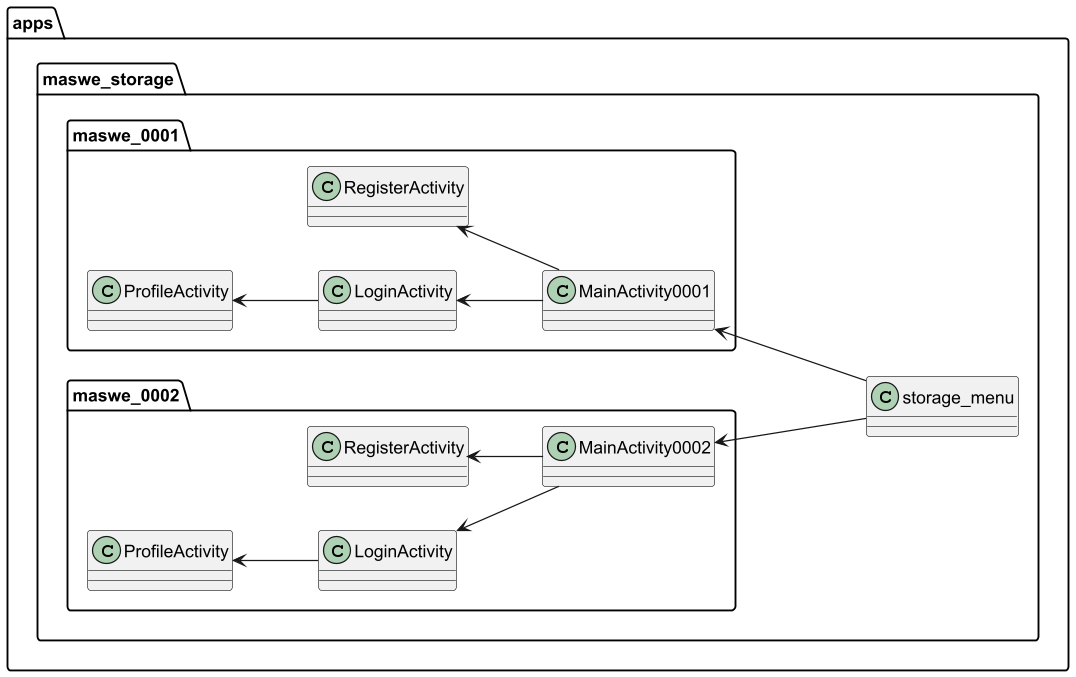
\includegraphics[width=1.0\textwidth]{dev_documents/BA_Thesis_Kronig/figures/diagrams/feature_oriented_approach_uml.png}
  \caption{ \todo{Add image caption} }
  \label{fig:label}
\end{figure}



\subsection{Template Based Activity-Architecture}
We make use of templates to heavily reduce the amount of boilerplate code. All of our vulnerability implementations require a starting as well as a register, login and profile activity, which differ in code logic but are (almost all) identical in layout. Because of this, the \texttt{common} library module includes four layout templates fitted with uniform styling and the basic navigating buttons and user input fields expected of them.  

The activities themselves share a lot of similarities and thus boilerplacte code as well. For example, many of the MASVS-CRYPTO vulnerabilities only differ in the concrete implementation of cryptographic operations, but are otherwise identical with each other as well as with vulnerabilities of other categories. To make use of these shared pieces of logic and remove redundancies, the \texttt{common} module includes three abstract activity templates that all activities make use of. The first is \texttt{BaseActivityTemplate.java} that all activities use, and the other two templates build on. The other two are \texttt{BaseRegisterActivity.java} \todo{fix spacing out of bounds here}and \texttt{BaseLoginActivity.java}.

\begin{figure}[htbp]
  \centering
  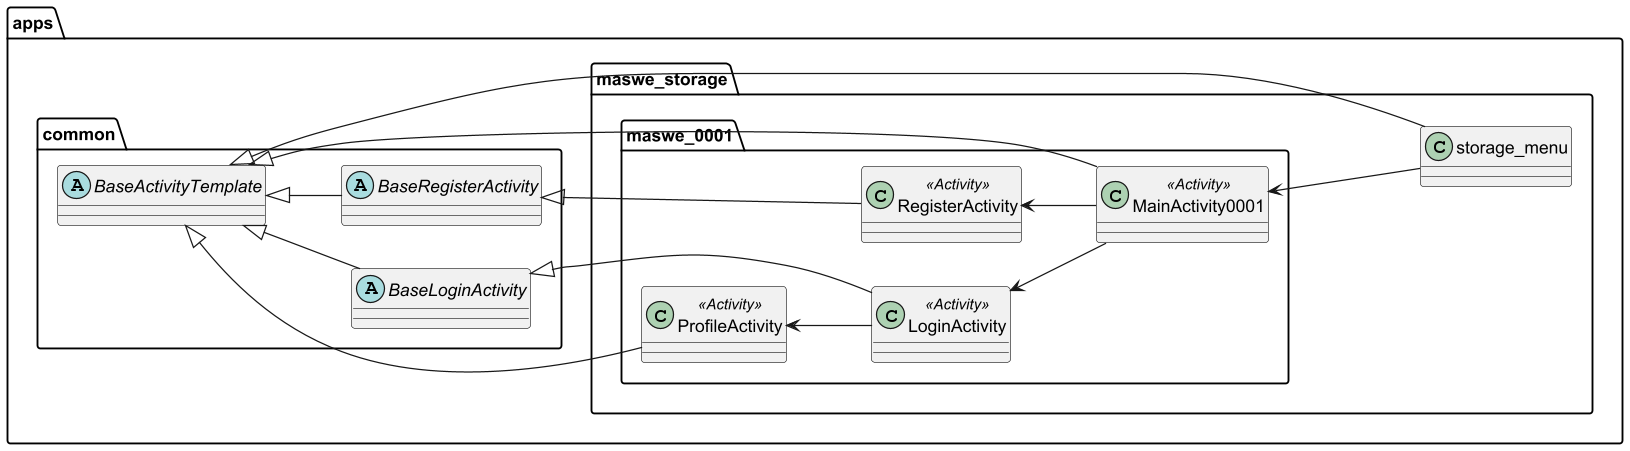
\includegraphics[width=1.0\textwidth]{dev_documents/BA_Thesis_Kronig/figures/diagrams/activity_templating_uml.png}
  \caption{ \todo{Add image caption} }
  \label{fig:label}
\end{figure}

\subsubsection{Base Activity Template}

\section{Models}
\subsection{UML Diagrams and Data Models}

\begin{figure}[htbp]
  \centering
  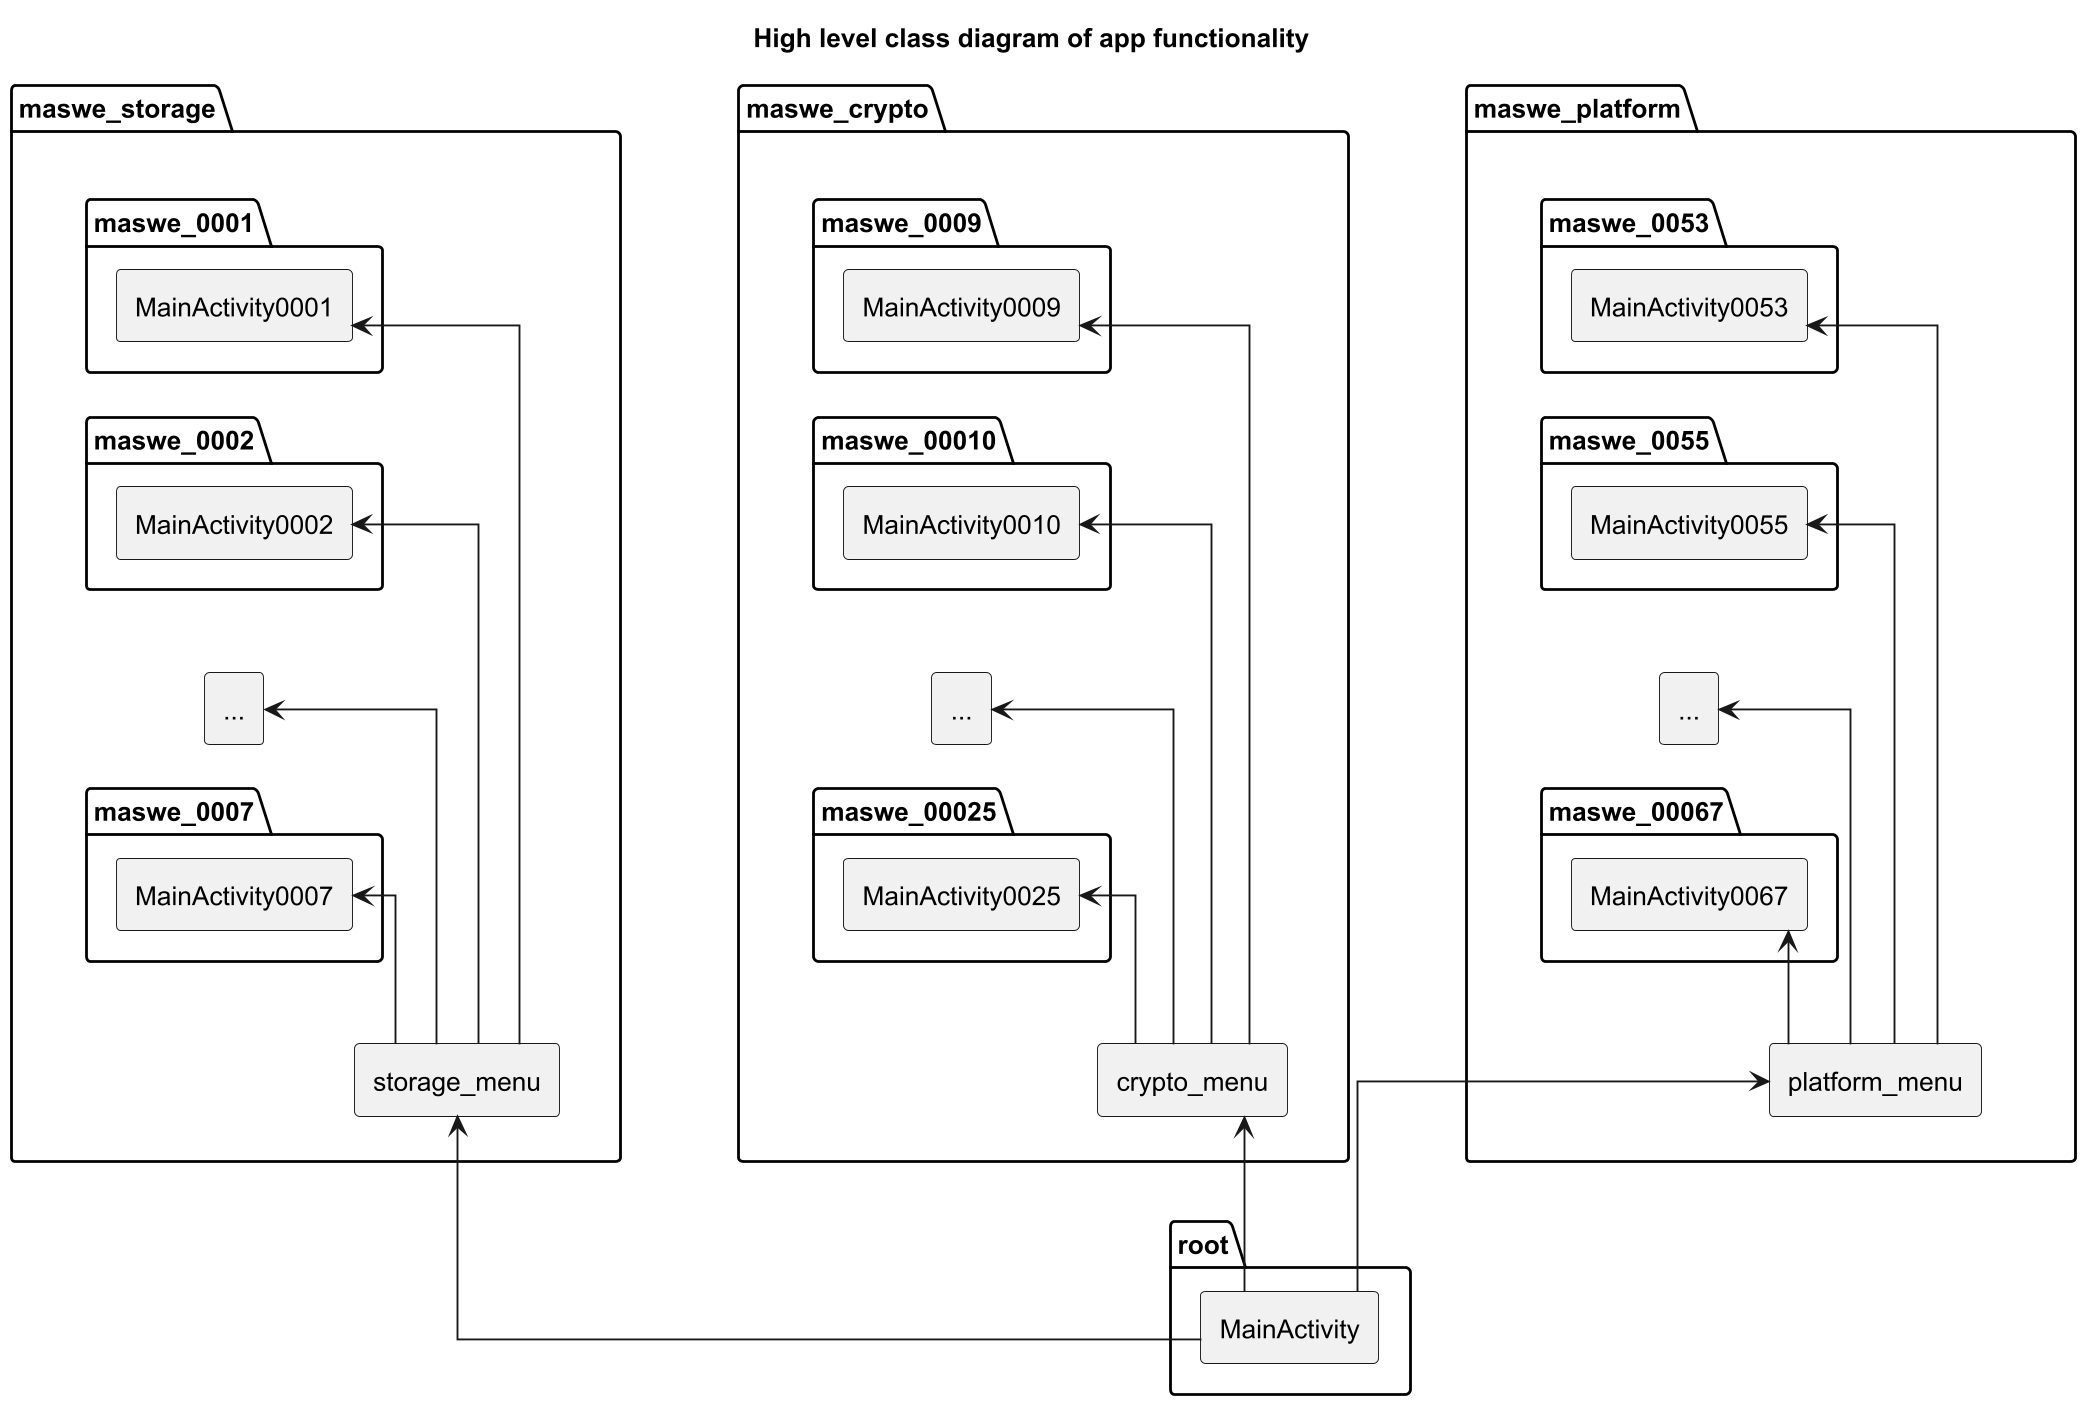
\includegraphics[width=1.0\textwidth]{dev_documents/BA_Thesis_Kronig/figures/diagrams/high_level_class_diagram_multiapp.png}
  \caption{ \todo{Add image caption} }
  \label{fig:label}
\end{figure}

\subsection{Use-Cases and Flow Diagrams}

\begin{figure}[htbp]
  \centering
  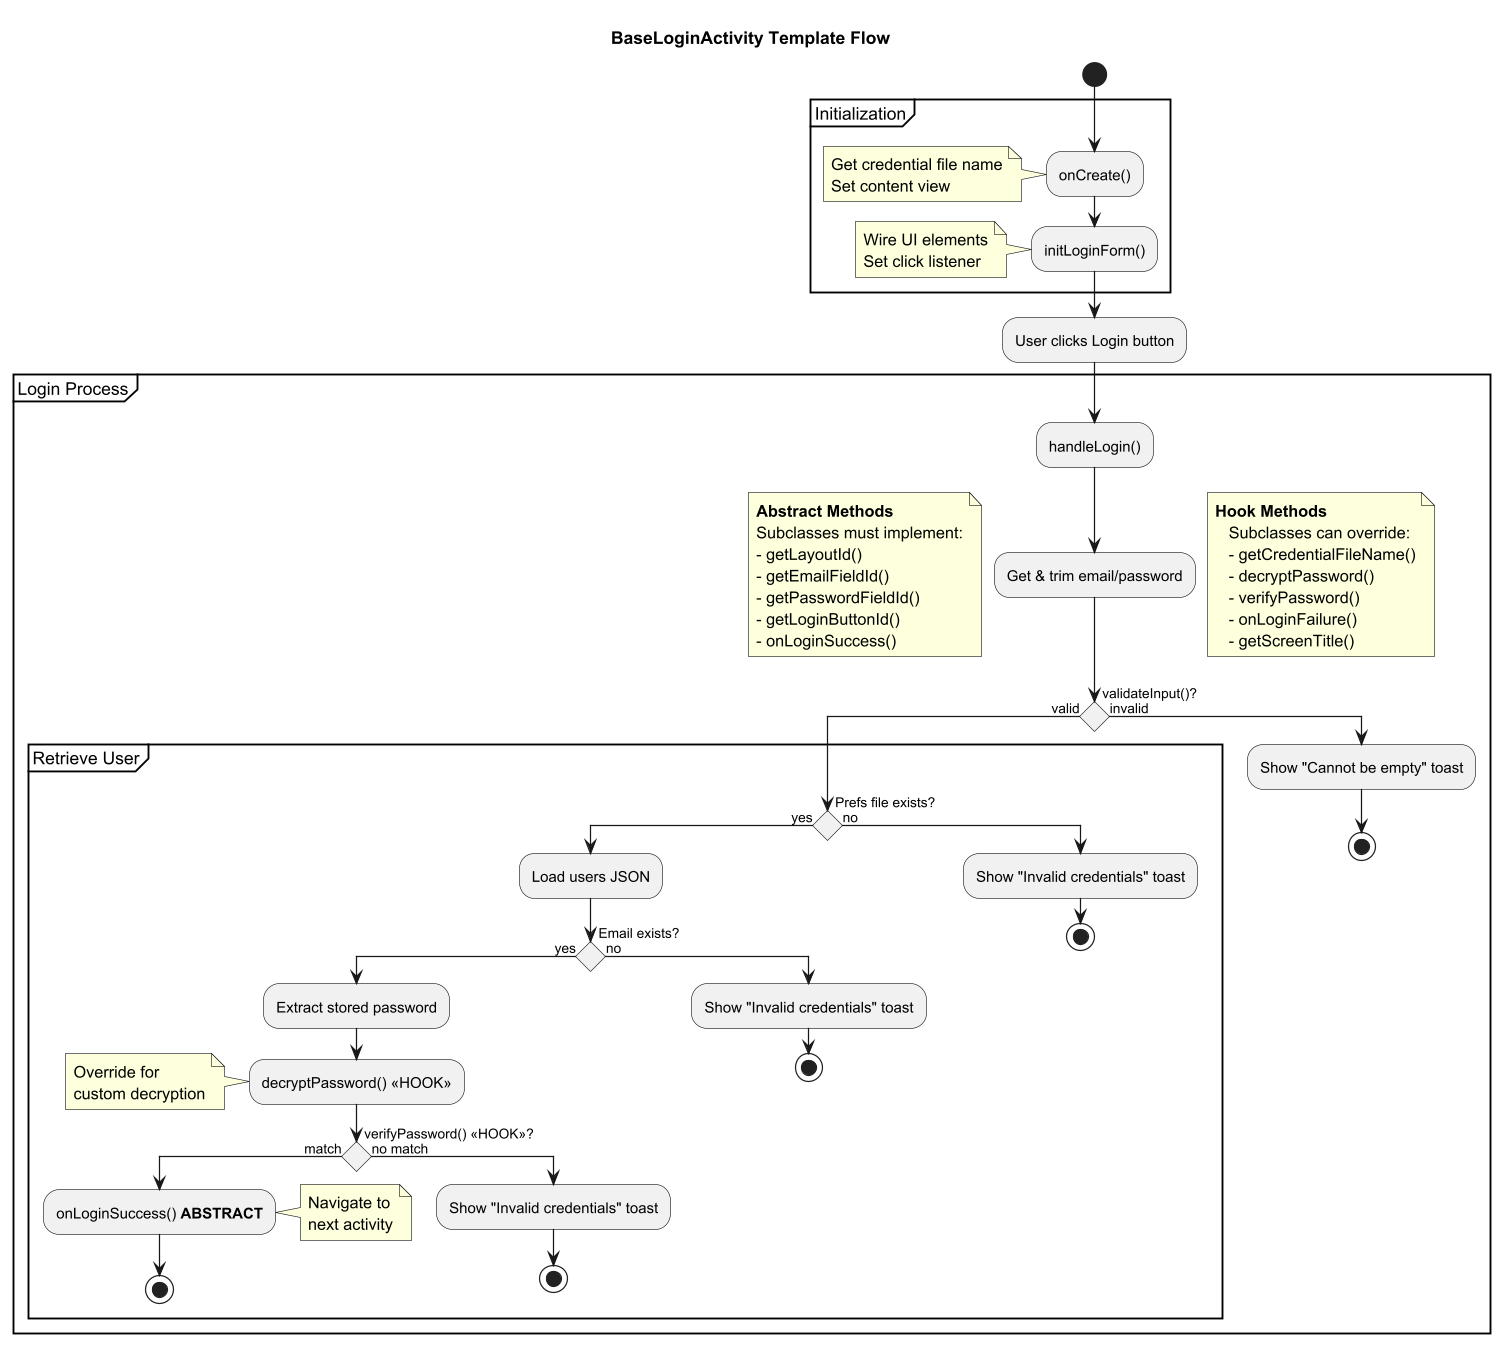
\includegraphics[width=1.0\textwidth]{dev_documents/BA_Thesis_Kronig/figures/diagrams/BaseLoginActivity_Template_Flow.png}
  \caption{ \todo{Add image caption} }
  \label{fig:label}
\end{figure}

\begin{figure}[htbp]
  \centering
  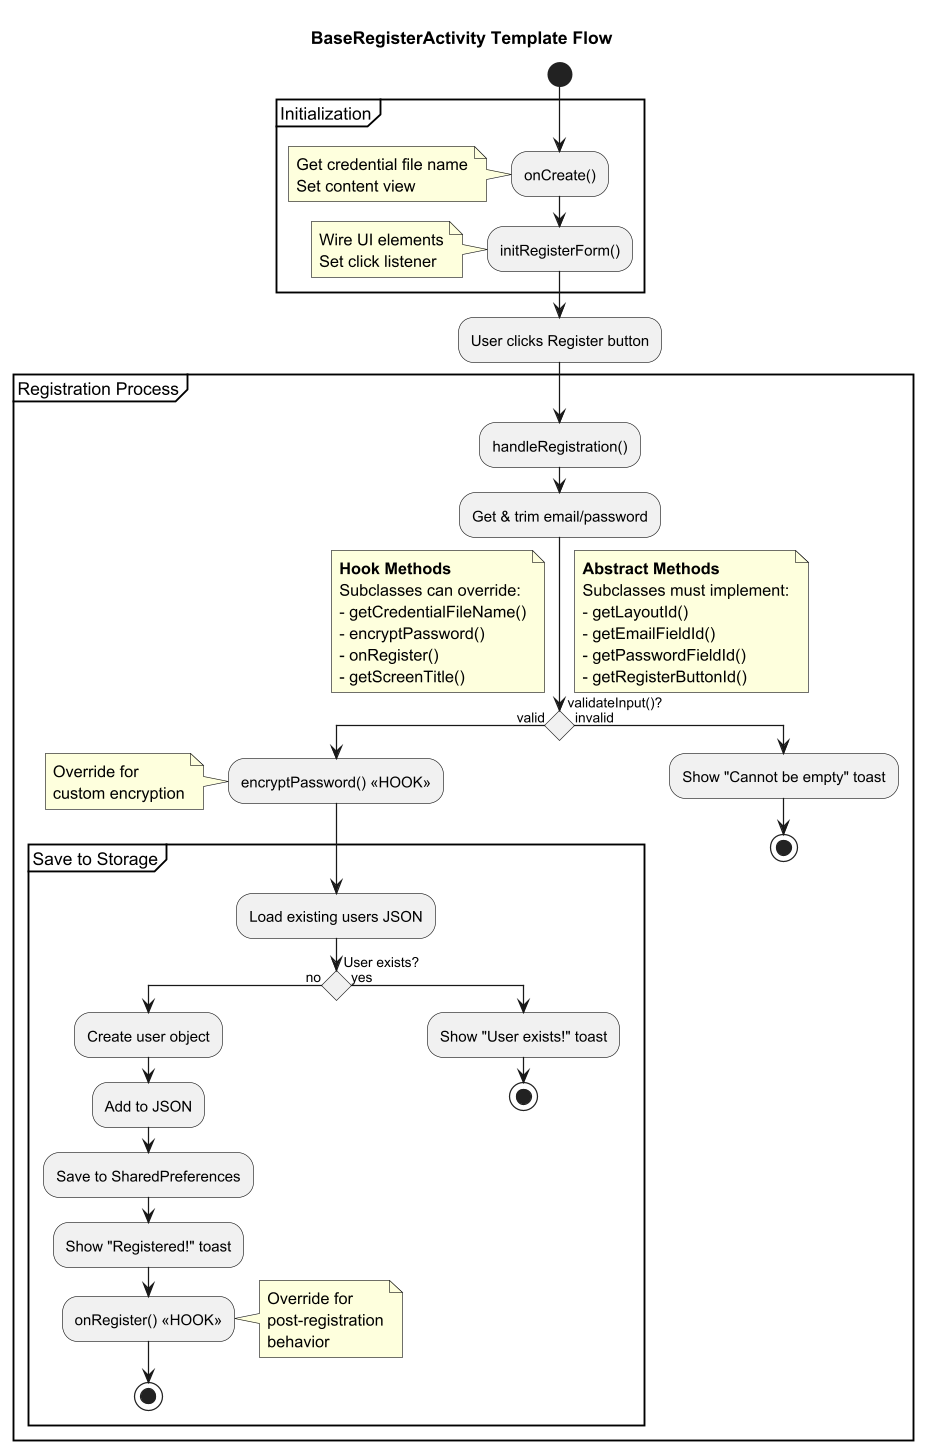
\includegraphics[width=1.0\textwidth]{dev_documents/BA_Thesis_Kronig/figures/diagrams/BaseRegisterActivity_Template_Flow.png}
  \caption{ \todo{Add image caption} }
  \label{fig:label}
\end{figure}

\begin{figure}[htbp]
  \centering
  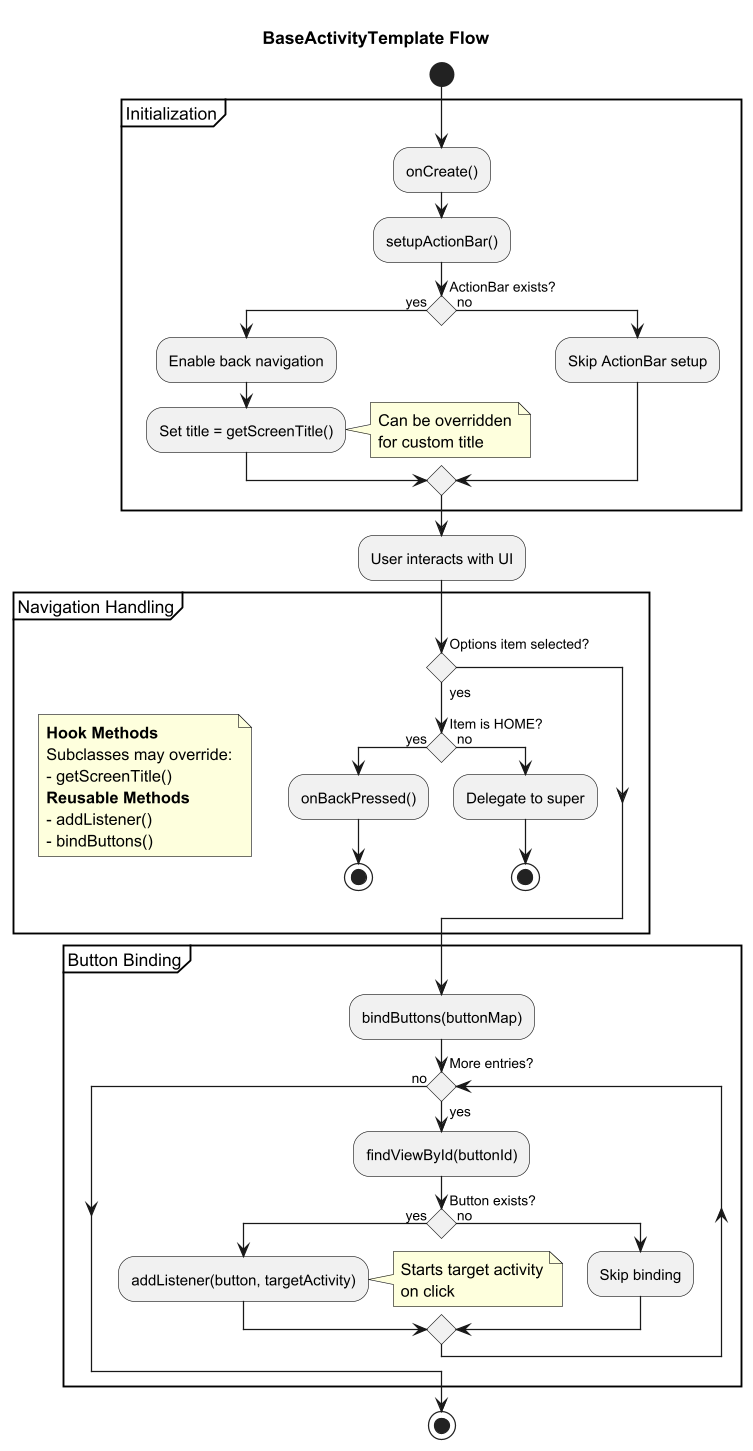
\includegraphics[width=1.0\textwidth, height=0.9\textheight, keepaspectratio]{dev_documents/BA_Thesis_Kronig/figures/diagrams/BaseActivityTemplate_Flow.png}
  \caption{ \todo{Add image caption} }
  \label{fig:label}
\end{figure}

\section{Vulnerabilities Selection Process}


\section{Design Decisions and Rationale}

\section{Considered Alternatives and Reasons for Rejection}